\documentclass[convert={outext=.png}]{standalone}
\usepackage{tikz}

\thispagestyle{empty}

\begin{document}
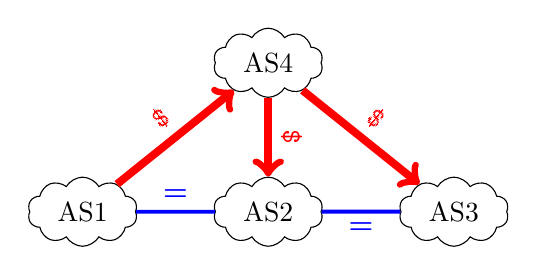
\begin{tikzpicture}
  \usetikzlibrary{positioning,matrix,arrows,shapes}

  [align=center,node distance=7cm]
   \tikzstyle{arrow} = [thick,->,>=stealth]
   \tikzset{router/.style = {rectangle, draw, text centered, minimum height=2em}, }
   \tikzset{host/.style = {circle, draw, text centered, minimum height=2em}, }
   \tikzset{ftable/.style={rectangle, dashed, draw} }
   \tikzset{as/.style={cloud, draw,cloud puffs=10,cloud puff arc=120, aspect=2, minimum height=1em, minimum width=1em} }
   \tikzset{state/.style={circle, draw, minimum height=2cm, minimum width=2cm} }
   \tikzset{pref/.style = {} }
   \node[as] (AS1) {AS1};
   \node[as, right =of AS1] (AS2) {AS2};
   \node[as, right =of AS2] (AS3) {AS3};
   \node[as, above = of AS2] (AS4) {AS4};

   
   % customer provider
   \draw[->, color=red, line width=1mm]
   (AS1) edge node [pos=0.5, sloped, above, color=red] {\texttt{\$}}(AS4)
   (AS4) edge node [pos=0.5, sloped, above, color=red] {\texttt{\$}}(AS2)
   (AS4) edge  node [pos=0.5, sloped, above, color=red] {\texttt{\$}} (AS3);
   \path[draw, color=blue, line width= .5 mm]
   (AS1) edge node [sloped, midway, above, color=blue] {\textbf{=}} (AS2)
   (AS2) edge node [sloped, midway, below, color=blue] {\textbf{=}} (AS3);

 
    

\end{tikzpicture}
\end{document}
